\documentclass[12pt]{article}

\usepackage{times}
\usepackage{graphicx}
\usepackage{amsmath}
\usepackage{url}
\usepackage{algorithmic}
\usepackage{enumerate}
\usepackage{float}

\setlength{\textwidth}{6.5in}
\setlength{\textheight}{8.9in}
\setlength{\oddsidemargin}{0.0in}
\setlength{\topmargin}{0.05in}
\setlength{\headheight}{-0.05in}
\setlength{\headsep}{0.0in}

\begin{document}

\begin{center}
{\bf CS 6300} \hfill {\large\bf HW10: Particle Filters and POMDPs \hfill Due April 27, 2017}
\end{center}

\noindent
Please use the \LaTeX\ template to produce your writeups. See the
Homework Assignments page on the class website for details.  Hand in
at: \url{https://webhandin.eng.utah.edu/index.php}.

\section{Particle Filtering}

PacBot is lost! It was exploring a maze when a solar storm occurred,
erasing its memory and leaving it with no information about where it
is. Luckily, the map of the maze was stored on its hard drive, and is
still available for PacBot to use.

\begin{center}
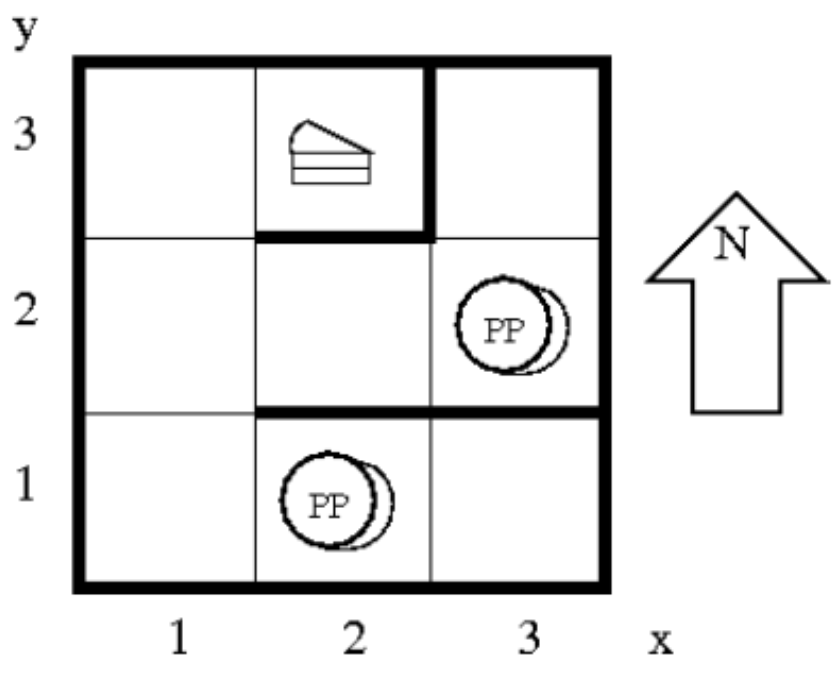
\includegraphics[width=0.4\textwidth]{prob1.png}
\end{center}

\noindent
PacBot decides to use particle filtering to figure out where it is. It
can make noise-free observations of the number of walls $W \in
\{1,2,3\}$, and noisy observations of food $F \in \{pie, power-pellet,
no-food\}$ at its current location.\newline
\newline
If there is food, it detects it correctly with probability
$\frac{3}{4}$, and detects nothing with probability $\frac{1}{4}$. An
example observation is (power-pellet, 2), which could occur in
locations (2,1) or (3,2).\newline
\newline
It chooses actions with the following probabilities: N: $\frac{1}{2}$,
S: $\frac{1}{6}$, E: $\frac{1}{6}$, W: $\frac{1}{6}$. In other words,
if you roll a standard 6 sided die and value is 1, 2, or 3 the
particle would move N, it would move S if the value was 4, E if the
value was 5, and W if the value was 6. If it tries to make a move and
bumps into a wall, it stays where it is, otherwise it moves with no
noise. \emph{Important:} When moving the particles start at the top
left and iterate row-by-row.

\begin{enumerate}[a)]

\item{Specify (i.e. give numbers for) the emission probabilities
  $P(E|X)$ associated with the HMM for this problem.}

\begin{table}[H]
\centering
\begin{tabular}{c r}
\hline\hline
$X$ & $P(E|X)$\\
\hline
$(1,1)$ & $P(\text{no food},2|X) = 1$\\
$(2,1)$ & $P(\text{no food},2|X) = 1/4$, $P(\text{power},2|X) = 3/4$\\
$(3,1)$ & $P(\text{no food},3|X) = 1$\\
$(1,2)$ & $P(\text{no food},1|X) = 1$\\
$(2,2)$ & $P(\text{no food},2|X) = 1$\\
$(3,2)$ & $P(\text{no food},2|X) = 1/4$, $P(\text{power},2|X) = 3/4$\\
$(1,3)$ & $P(\text{no food},2|X) = 1$\\
$(2,3)$ & $P(\text{no food},3|X) = 1/4$, $P(\text{pie},3|X) = 3/4$\\
$(3,3)$ & $P(\text{no food},3|X) = 1$\\
\hline
\end{tabular}
\end{table}

\item PacBot starts doing particle filtering with 9 particles, one in
  each location.  Perform a single \emph{time} step of particle
  filtering and indicate where particles moved, using the following
  random numbers in order: (4, 1, 5, 5, 2, 6, 1, 6, 2).  For example,
  particle 1 is in $(x,y) = (1,3)$ and will move (or not) to some
  other square which you'll indicate with a table.

\begin{table}[H]
\centering
\begin{tabular}{c c}
\hline\hline
$X(t_{0})$ & $X(t_{1})$\\
\hline
$(1,1)$ & $(1,1)$\\
$(2,1)$ & $(2,1)$\\
$(3,1)$ & $(3,1)$\\
$(1,2)$ & $(2,2)$\\
$(2,2)$ & $(2,2)$\\
$(3,2)$ & $(2,2)$\\
$(1,3)$ & $(1,3)$\\
$(2,3)$ & $(1,3)$\\
$(3,3)$ & $(3,3)$\\
\hline
\end{tabular}
\end{table}

\item PacBot now makes the observation (no-food, 3).  Complete the
    evidence step of particle filtering. \emph{Re-weight} your
    particles from step (b), and normalize them based on the sum of
    all weights * 9.

\begin{table}[H]
\centering
\begin{tabular}{c c}
\hline\hline
$X(t_{1})$ & $w(X)$\\
\hline
$(3,1)$ & $1/18$\\
$(3,3)$ & $1/18$\\
\hline
\end{tabular}
\end{table}

The rest of the weights are $0$


\item Now re-sample the particles with 9 new, equally weighted (1.0)
  particles.  To do the re-sampling, use the following
  pseudo-code:

   \begin{algorithmic}
   \FOR{$i=1 \rightarrow 9$}
      \STATE $rand \leftarrow rand[0,9]$
      \STATE $sum \leftarrow  0$
      \FOR{ all weighted (normalized) particles $j$ }
         \STATE $sum \leftarrow sum + $ weight of particle $j$
         \IF { $sum \ge rand$ }
            \STATE place a new particle onto new map at this particle's location
            \STATE $break$
         \ENDIF
      \ENDFOR
   \ENDFOR
   \end{algorithmic}

   To help you with the sampling, here are 9 randomly generated
   numbers between 1 and 9: (2, 9 , 1, 4, 9, 5, 6, 3, 4). Assign
   values from this probability distribution in ascending order and
   assign them to cells from left-to-right, top-to-bottom.

\item{What do the particles look like after another \emph{time} step?
    Here are 9 uniformly, randomly chosen numbers between 1 and 6: (4,
    3, 1, 5, 3, 6, 3, 6, 5)}

\end{enumerate}

\clearpage

\section{POMDP}

An agent is in one of the two cells $s_1,s_2$.  There are two actions
$a \in \{ go, stay\}$: the agent can either stay in the cell, or
attempt to go to the other cell.  The transition probabilities
$T(s_i,a,s_j)$ (take action $a$ from state $s_i$ and arrive in state
$s_j$) are:

\begin{center}
\begin{tabular}{l}
$T(s_i,stay,s_j) = \left\{ \begin{array}{lll}
                                   0 & \hbox{for} & i\neq j \\
                                   1 & \hbox{for} & i = j
                            \end{array}
                    \right.$ \\[.2in]
$T(s_i,go,s_j) = \left\{ \begin{array}{lll}
                                   0.25 & \hbox{for} & i\neq j \\
                                   0.75 & \hbox{for} & i = j
                            \end{array}
                    \right.$
\end{tabular}
\end{center}

\noindent
The reward function has the simplified form $R(s_i,a,s_j) = R(s_j)$,
i.e., it depends only on the state you end up in.  There is a reward
for transitioning to state $s_2$, but none to state $s_1$:

$$R(s_2) = 1, \quad R(s_1) = 0$$

\noindent
The agent has an ultrasound sensor which helps to distinguish which
cell it's in.  There are two possible readings $z_1$ or $z_2$
corresponding to an estimation of being in cell $s_1$ or $s_2$
respectively, but the sensor is noisy and sometimes gives the wrong
reading.  Its conditional probability is given by:

$$P(z_i | s_j) = \left\{ \begin{array}{lll}
                                   0.2 & \hbox{for} & i\neq j \\
                                   0.8 & \hbox{for} & i = j
                            \end{array}
                    \right.$$

\noindent
The agent maintains and updates a belief function $b(s_i)$ based upon
combinations of actions and associated sensor readings.  For brevity,
define $p_1 = b(s_1)$.  Hence $b(s_2) = 1 - p_1$.

\begin{enumerate}

\item For the first action and without receiving any sensor readings
  yet, derive the one-time-step utilities $V^{stay}(s_i)$ and
  $V^{go}(s_i)$, $i=1,2$, for actions $stay$ and $go$.

\item You don't actually know which state you're in, and you have to
  use your belief function $b(s_i)$ to combine the results above.
  Find the expected reward $V(b,go)$ for action $go$, and $V(b,stay)$
  for action $stay$.

\item Plot both expected reward functions on the same plot with $p_1$
  on the x-axis.  Identify the optimal strategy based on your plot.

\item Suppose you are able to get a sensor reading before taking an
  action, and you observe $z_1$.  Update your belief to find $p(s_1 |
  z_1)$ and $p(s_2 | z_1)$.

\item Solve for the new value functions given $b'$.

\end{enumerate}
 
\end{document}


